\chapter{Playing With Lines}

The method of least squares is a wonderfully versatile tool, and we will get a sense of this from looking at the canonical equation for a line
  \begin{equation*}   %  =   =   =   =   =
   %\begin{split}
      y(x) = a_{0} + a_{1} x.
   %\end{split}
   %\label{eq:}
  \end{equation*}
There are two ways to exploit the equation. One way is to input a set of measurements $\lst{x_{k},y_{k}}_{k=1}^{m}$, and find the best parameters $\paren{a_{0},a_{1}}$, in the least squares sense. 

The focus on this chapter is to start with a set of parameters $\paren{a_{0},a_{1}}$ and to find the best set $\paren{x, y}$, in the least squares sense.	

\begin{table}[htbp]  % + + + + T A B L E
    \caption{Given the parameters for a line find the solution locus.}
    \begin{center}
        \begin{tabular}{lcl}
            %
            input & $\rightarrow$ & output \\\hline
            %
            parameters $a_{0}$, $a_{1}$ && set $(x, y)$\\
      		%
			intercept, slope && least squares solution
            %
        \end{tabular}
    \end{center}
    %\label{default}
\end{table}%


\section{A Single Line}  %    S    S    S    S    S    S    S    S    S

Given the parameters $a=\mat{c}{a_{0}\\a_{1}}$, find the set $\mat{c}{x\\y}$ which comprises the least squares solution for
  \begin{equation}   %  =   =   =   =   =
   %\begin{split}
      y = a_{0} + a_{1} x, \qquad a_{0} \ne 0.
   %\end{split}
   \label{eq:myline}
  \end{equation}

\begin{figure}[htbp] %  figure placement: here, top, bottom, or page
   \centering
   \begin{overpic}[ scale = \myscale ]
	   {\pathgraphics tricks/one_line/"line- y = mx + b"}
        %
    	\put(50,-3) {$x$}
    	\put(-4,31) {$y$}
	    %
   \end{overpic}
   \caption{A sample line.}
   %\label{fig:three lines oval}
\end{figure}

Rewriting \eqref{eq:myline} as a linear system reveals
  \begin{equation*}   %  =   =   =   =   =
   %\begin{split}
      -a_{1} x + y = a_{0},
   %\end{split}
   %\label{eq:}
  \end{equation*}
which is the linear system
  \begin{equation}   %  =   =   =   =   =
  %\begin{split}
    \mat{rc}{ -a_{1} & 1 } \mat{c}{x\\y} = \mat{c}{a_{0}}.
    \label{eq:one line problem}
  %\end{split}
  \end{equation}
Certainly, the heavy artillery of the SVD could be brought to bear. Yet simple geometric reasoning will produce a solution and reinforce basic insights. The SVD will then be a trivial exercise.

Equation \eqref{eq:myline} describes a line, a continuous set of points. Referring back to the boxed least squares solution in \eqref{eq:general soln}, the least squares solution may be the 

Which point on the line is closet to the origin? One way to solve for this is use the fact that the shortest line through the origin which connects with \eqref{eq:myline} is perpendicular to \eqref{eq:myline}. This is the orthogonal projection theorem.

  \begin{table}[h]  %  T A B L E
    \caption{Problem statement for least squares solution for a single line.}
    \begin{center}
      \begin{tabular}{lll}
        %
        \bf{trial function} & $y(x) = a_{0} + a_{1} x$ \\
        \bf{residual error} & $r(x) = y - a_{0} - a_{1} x$ \\
        \bf{merit function} & $M(a) = \paren{y - a_{0} - a_{1} x}^{2}$\\
        \bf{inputs}         & $a_{0}$ & $y-$axis intercept \\
                            & $a_{1}$ & slope \\
        \bf{results}        & $\mat{c}{x\\y}_{LS} = \bl{\mat{c}{x\\y}_{part}} + \rd{\mat{c}{x\\y}_{homog}}$   \\
        \bf{\# of parameter sets} & $m = 1$ & rows in $\A{}$ \\
        \bf{\# of parameters}   & $n = 2$ & columns in $\A{}$ \\
        \bf{system matrix}  & $\A{} \in \real{1 \times 2}_{1}$ \\
        \bf{linear system}  & $\mat{cc}{-a_{1} & 1} 
                               \mat{c}{x \\ y} = 
                               \mat{c}{a_{0}}$ \\
        %\bf{ideal solution} & NA \\
        \bf{input data}     & $a_{0}$, $a_{1}$
        %
      \end{tabular}
    \end{center}
  \label{tab:one line inputs}
  \end{table}%

\begin{figure}[htbp] %  figure placement: here, top, bottom, or page
   \centering
   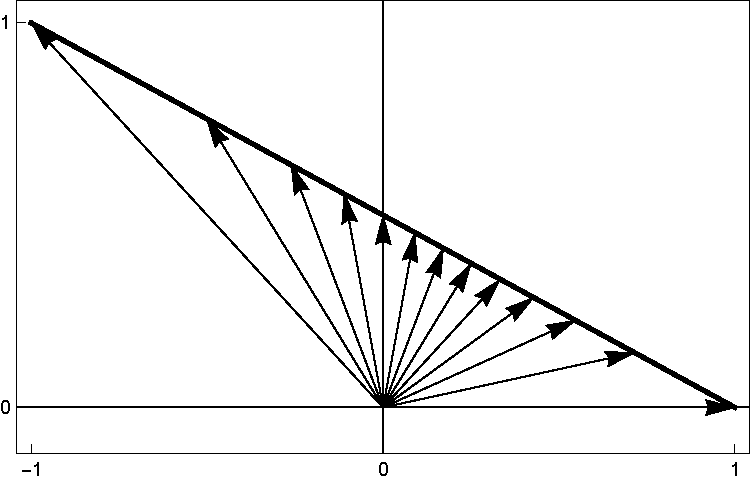
\includegraphics[ width = 3.5in ]{\pathgraphics tricks/one_line/fan} 
   \caption{Every point on the line satisfies the least squares criterion; the particular solution is the vector of minimum length.}
   %\label{fig:example}
\end{figure}

  \begin{equation*}   %  =   =   =   =   =
   %\begin{split}
      \mat{cc}{-a_{1} & 1} 
      \mat{c}{x\\y} =
      \mat{c}{a_{0}}
   %\end{split}
   %\label{eq:}
  \end{equation*}
  \begin{equation*}   %  =   =   =   =   =
   %\begin{split}
      x_{LS} = \lst{x\in\real{2}\colon \norms{\A{}x - a_{0}} \text{is minimized}}
   %\end{split}
   %\label{eq:}
  \end{equation*}
  \begin{equation*}   %  =   =   =   =   =
   %\begin{split}
      M\paren{x,y} = \paren{ - a_{1} x + y - a_{0}}^{2}
   %\end{split}
   %\label{eq:}
  \end{equation*}

\begin{figure}[htbp] %  figure placement: here, top, bottom, or page
   \centering
   \begin{overpic}[ scale = \myscale ]
	   {\pathgraphics tricks/one_line/"one line merit"}
	    %
	    \put(25,55) {$M(a_{0},a_{1}) = \paren{y - a_{0} - a_{1}x}^{2}$}
        %
    	\put(50,-3) {$x$}
    	\put(-4,27) {$y$}
	    %
   \end{overpic}
   \caption{A contour plot of the merit function showing the particular solution (blue dot) and homogeneous solution (red dashes).}
   \label{fig:one lines merit}
\end{figure}

\subsection{Geometric Solution}  %    SS    SS    SS    SS    SS    SS    SS    SS    SS
Every point on the line \eqref{eq:myline} is a point of 0 residual, therefore every point on the line is a solution point. 

The least squares solution is the solution of minimum length.
  \begin{equation*}   %  =   =   =   =   =
   %\begin{split}
      y = -\frac{1}{a_{1}} x
   %\end{split}
   %\label{eq:}
  \end{equation*}
    \begin{equation*}   %  =   =   =   =   =
   %\begin{split}
      x = \frac{a_{0} a_{1}} {\onelen}
   %\end{split}
   %\label{eq:}
  \end{equation*}

  \begin{equation*}   %  =   =   =   =   =
   %\begin{split}
      \mat{c}{x\\y}_{LS} = \frac{a_{0}} {1 + a_{1}^{2}} \mat{c}{-a_{1}\\1}
   %\end{split}
   %\label{eq:}
  \end{equation*}
    
  \begin{equation*}   %  =   =   =   =   =
   %\begin{split}
      p(\tau) = p_{0} + \tau \mat{c}{1\\a_{1}}
   %\end{split}
   %\label{eq:}
  \end{equation*}

  \begin{equation*}   %  =   =   =   =   =
   %\begin{split}
      \mat{c}{x\\y}_{LS} = \frac{a_{0}} {1 + a_{1}^{2}} 
        \bl{\mat{c}{-a_{1}\\1}} +
        \tau \rd{\mat{c}{1\\a_{1}}}
   %\end{split}
   %\label{eq:}
  \end{equation*}

  \begin{equation}   %  =   =   =   =   =
      \A{\dagger} a_{0} = \frac{a_{0}}{\onelen} \mat{c}{-a_{1} \\ 1}
   \label{eq:one line soln}
  \end{equation}

Every point on the line in \eqref{eq:myline}

\begin{figure}[htbp] %  figure placement: here, top, bottom, or page
   \centering
   \begin{overpic}[ scale = \myscale ]
	   {\pathgraphics tricks/one_line/"line- blue dot, red line"}
        %
        \put(17,42) {\rd{$x_{homog}$}}
        \put(27,48) {\rd{$\pna z$}}
        %
        \put(50,25) {\colorbox{white}{\bl{$x_{part}$}}}
        \put(61,31) {\bl{$\Ap a_{0}$}}
        %
    	\put(50,-3) {$x$}
    	\put(-4,31) {$y$}
	    %
   \end{overpic}
   \caption{The least squares solution for \eqref{eq:one line problem} resolved into range space (blue) and null space components (red).}
   \label{fig:one line resolved}
\end{figure}

  \begin{table}[t]  %  T A B L E
    \caption{Results for best line with $a_{0} = \frac{1}{2}$, $a_{1} = -\frac{1}{2}$.}
    \begin{center}
      \begin{tabular}{lll}
        %
        \bf{input parameters} & $a_{0} =  \frac{1}{2}$ & intercept \\
                              & $a_{1} = -\frac{1}{2}$ & slope \\
        \bf{computed solution} & $\mat{c}{x\\y}_{LS} = \bl{\frac{1}{5}\mat{c}{1\\2}} + \tau \rd{\mat{c}{1\\-1/2}}$ & $\tau \in \cmplx{}$\\
        \bf{solution error} & 0 & exact solution \\
        \bf{ideal solution} & $\mat{c}{ \tilde{a}_{0} \\ \tilde{a}_{1} } = \mat{c}{0\\10}$ \\
        \bf{$\rtr{*}$} & $0$ \\
        \bf{curvature matrix $\wxi{*}$} & $\frac{1}{4}\mat{rr}{1 & \mg{2} \\ \mg{2} & 4 }$\\[5pt]
        \bf{problem statement} & table \ref{tab:one line inputs} \\
        %\bf{input data}        & table \ref{tab:bevington data and results} \\
        \bf{plots}             & figure \ref{fig:one line resolved} & 1. solution\\
           & figure \ref{fig:one lines merit} & 2. merit function \\
        %
      \end{tabular}
    \end{center}
  \label{tab:one line solution}
  \end{table}%

\subsection{SVD}  %    SS    SS    SS    SS    SS    SS    SS    SS    SS
We can construct the \asvd \ by inspection. The target matrix $\A{} = \mat{cc}{-a_{1} & 1}$ has 1 row, which implies the matrix for the codomain is
  \begin{equation*}   %  =   =   =   =   =
   %\begin{split}
      \U{} = \mat{c}{1}.
   %\end{split}
   %\label{eq:}
  \end{equation*}
The 

  \begin{equation*}   %  =   =   =   =   =
    \begin{array}{ccccc}
      %
      \A{} &=& \U{} & \Sigma & \V{*} \\
      %
      \mat{cc}{-a_{1} & 1} &=& 
      \mat{c}{1} & 
      \mat{cc}{\sqrt{\onelen} & 0} & 
      \frac{1}{\onelensq}
      \mat{cc}{\bl{-a_{1}} & \bl{1} \\ \rd{1} & \rd{a_{1}} }
      %
    \end{array}
   %\label{eq:}
  \end{equation*}

  \begin{equation*}   %  =   =   =   =   =
   %\begin{split}
      \Ap = \V{} \sig{\sym} \U{*} = \frac{1} {\onelen} \mat{c}{-a_{1} \\ 1}
   %\end{split}
   %\label{eq:}
  \end{equation*}
Compare $\Ap a_{0}$ to \eqref{eq:one line soln}.

\section{Two Lines}  %    S    S    S    S    S    S    S    S    S
Where Do Parallel Lines Cross? The provocative question which opens this section has an obvious answer in Euclidean space. There is no such point; parallel lines never cross. Yet, if we input these lines as a linear system, we compute a least squares solution. What is the significance of the least squares solution?

Consider this tantalizing example. The two lines,
  \begin{equation*}   %  =   =   =   =   =
    \begin{split}
      y(x) &= \half - \half x, \\
      y(x) &= 1 - \half x,
    \end{split}
   %\label{eq:}
  \end{equation*}
are plotted in figure \ref{fig:tantalizing} along with the least squares solution is 
  \begin{equation*}   %  =   =   =   =   =
   %\begin{split}
      x_{LS} = \Ap b = \frac{1}{10}\mat{c}{ 3 \\ 6}.
   %\end{split}
   %\label{eq:}
  \end{equation*}
What is so special about this point?
\begin{figure}[htbp] %  figure placement: here, top, bottom, or page
   \centering
     \includegraphics[ width = 3in ]{\pathgraphics "tricks"/two_lines/"parallel point"} 
   \caption{Parallel lines and the least squares solution.}
   \label{fig:tantalizing}
\end{figure}

\subsection{Intersecting Lines}
  \begin{equation*}   %  =   =   =   =   =
   \begin{split}
      y &= 1, \\
      y &= x .
   \end{split}
   %\label{eq:}
  \end{equation*}

  \begin{equation*}   %  =   =   =   =   =
   %\begin{split}
      \mat{rr}{0 & 1 \\ -1 & 1 }\mat{c}{x\\y} = \mat{c}{1\\0}
   %\end{split}
   %\label{eq:}
  \end{equation*}


\section{Three Lines}  %    S    S    S    S    S    S    S    S    S
Start with three distinct lines. The first line represents a constant value. The second line has a fixed slope, the third has a variable slope. We will study how the solution varies as this slope $m$ is varied.
  \begin{equation*}   %  =   =   =   =   =
     \begin{split}
       %
       y_{1}(x) &= 1, \\
       y_{2}(x) &= 1 - x, \\
       y_{3}(x) &= m x.
       %
     \end{split}
   %\label{eq:}
  \end{equation*}

%  \begin{equation*}   %  =   =   =   =   =
%    \begin{split}
%      &y = 1 \\
%      x + &y = 1 \\
%      -mx +&y = 0
%    \end{split}
%   %\label{eq:}
%  \end{equation*}

  \begin{table}[htbp]
  \caption{Rewriting the equations $y=mx+b$ as a linear system.}
  \begin{center}
    \begin{tabular}{lclcccrcrcl}
      %
      $y_{1}(x)$ &=&  1       && $\Rightarrow$ && &&          $y$ &=& 1 \\
      %
      $y_{2}(x)$ &=&  $1 - x$ && $\Rightarrow$ && $x$   & + & $y$ &=& 1 \\
      %
      $y_{3}(x)$ &=&  $m x$   && $\Rightarrow$ && $-mx$ & + & $y$ &=& 0 \\
      %
    \end{tabular}
  \end{center}
  %\label{default}
  \end{table}%


  \begin{equation*}   %  =   =   =   =   =
   %\begin{split}
      \mat{rc}{0 & 1 \\ 1 & 1 \\ -m & 1 } 
      \mat{c}{x \\ y} = 
      \mat{c}{1\\1\\0}
   %\end{split}
   %\label{eq:}
  \end{equation*}

Merit function
  \begin{equation*}   %  =   =   =   =   =
   %\begin{split}
      M(x,y) = \normts{\A{}\mat{c}{x\\y}-b}
   %\end{split}
   %\label{eq:}
  \end{equation*}

  \begin{equation*}   %  =   =   =   =   =
   %\begin{split}
      \A{*} \cdot \A{} = 
      \mat{lc}{1+m^{2} & 1-m \\ 1-m & 3}
   %\end{split}
   %\label{eq:}
  \end{equation*}

  \begin{equation*}   %  =   =   =   =   =
    \begin{split}
      \tr {\A{}} &= 4 + m^{2} \\
      \det \paren{\A{}} &= 2 + 2m + 2m^{2}
    \end{split}
   %\label{eq:}
  \end{equation*}

  \begin{equation*}   %  =   =   =   =   =
   %\begin{split}
      p\paren{\lambda} = \lambda^{2} - \lambda \, \tr{\W{}} + \det\paren{\W{}}
   %\end{split}
   %\label{eq:}
  \end{equation*}
  \begin{equation*}   %  =   =   =   =   =
   %\begin{split}
      p\paren{\lambda} = 0
   %\end{split}
   %\label{eq:}
  \end{equation*}

  \begin{equation*}   %  =   =   =   =   =
   %\begin{split}
      \lambda_{\pm} = \frac{\tr{\W{}} \pm \sqrt{ \tr{\W{}}^{2} - 4 \det\paren{\W{}} } } {2}
   %\end{split}
   %\label{eq:}
  \end{equation*}


  \begin{equation*}   %  =   =   =   =   =
   %\begin{split}
      \sigma = 2^{-1/2} \sqrt{m^{2} + 4 \pm \factor}
   %\end{split}
   %\label{eq:}
  \end{equation*}

  \begin{equation*}   %  =   =   =   =   =
      \xi = \factor
   %\label{eq:}
  \end{equation*}

%\begin{table}[htbp]
%\caption{Least squares solution for three distinct lines as the parameter $m$ varies from 0 to $\infty$.}
%    \begin{center}
%        \begin{tabular}{ccc}
%           %
%           & Domain: Graphs & Domain: Merit Function \\\hline
%           %
%           \raisebox{1.5\height}{$m=0$} &
%           \includegraphics[ width = 2in ]{\pathgraphics tricks/three_lines/"three lines m = 0"} &
%           \includegraphics[ width = 2.1in ]{\pathgraphics tricks/three_lines/"merit function m = 0"} \\[10pt]
%           %
%           \raisebox{-2.5\height}{$m=1$} &
%           \includegraphics[ width = 2in ]{\pathgraphics tricks/three_lines/"three lines m = 1"} &
%           \includegraphics[ width = 2.1in ]{\pathgraphics tricks/three_lines/"merit function m = 1"} \\[10pt]
%           %
%           $m=2$ &
%           \includegraphics[ width = 2in ]{\pathgraphics tricks/three_lines/"three lines m = 2"} &
%           \includegraphics[ width = 2.1in ]{\pathgraphics tricks/three_lines/"merit function m = 2"} \\[10pt]
%           %
%           $m=5$ &
%           \includegraphics[ width = 2in ]{\pathgraphics tricks/three_lines/"three lines m = 5"} &
%           \includegraphics[ width = 2.1in ]{\pathgraphics tricks/three_lines/"merit function m = 5"} \\[10pt]
%           %
%           $m=\infty$ &
%           \includegraphics[ width = 2in ]{\pathgraphics tricks/three_lines/"three lines m = inf"} &
%           \includegraphics[ width = 2.1in ]{\pathgraphics tricks/three_lines/"merit function m = inf"} \\
%           %
%        \end{tabular}
%    \end{center}
%\label{tab:three lines}
%\end{table}%

\break
\begin{table}[htbp]
\caption{Least squares solution for three distinct lines as the parameter $m$ varies from 0 to $\infty$.}
    \begin{center}
        \begin{tabular}{lc}
           %
           $m$ & Domain: Graphs \\\hline
           %
           \raisebox{8\height}{$m=0$} &
           \includegraphics[ width = 2.5in ]{\pathgraphics tricks/three_lines/"three lines m = 0"} \\[7pt]
           %
           \raisebox{8\height}{$m=1$} &
           \includegraphics[ width = 2.5in ]{\pathgraphics tricks/three_lines/"three lines m = 1"}\\[7pt]
           %
           \raisebox{8\height}{$m=5$} &
           \includegraphics[ width = 2.5in ]{\pathgraphics tricks/three_lines/"three lines m = 5"}\\[7pt]
           %
           \raisebox{12\height}{$m=\infty$} &
           \includegraphics[ width = 2.5in ]{\pathgraphics tricks/three_lines/"three lines m = inf"}
           %
        \end{tabular}
    \end{center}
\label{tab:three lines graphs}
\end{table}%

\begin{table}[htbp]
\caption{Least squares solution for three distinct lines as the parameter $m$ varies from 0 to $\infty$.}
    \begin{center}
        \begin{tabular}{lc}
           %
           $m$ & Domain: Merit function \\\hline
           %
           \raisebox{8\height}{$m=0$} &
           \includegraphics[ width = 2.5in ]{\pathgraphics tricks/three_lines/"merit function m = 0"} \\[7pt]
           %
           \raisebox{8\height}{$m=1$} &
           \includegraphics[ width = 2.5in ]{\pathgraphics tricks/three_lines/"merit function m = 1"}\\[7pt]
           %
           \raisebox{8\height}{$m=5$} &
           \includegraphics[ width = 2.5in ]{\pathgraphics tricks/three_lines/"merit function m = 5"}\\[7pt]
           %
           \raisebox{12\height}{$m=\infty$} &
           \includegraphics[ width = 2.5in ]{\pathgraphics tricks/three_lines/"merit function m = inf"}
           %
        \end{tabular}
    \end{center}
\label{tab:three lines merit}
\end{table}%

%\begin{landscape}
%\begin{table}[htbp]
%\caption{Least squares solution for three distinct lines as the parameter $m$ varies from 0 to $\infty$.}
%    \begin{center}
%        \begin{tabular}{ccc}
%           %
%           & Domain: Graphs & Domain: Merit Function \\\hline
%           %
%           \raisebox{10\height}{$m=0$} &
%           \includegraphics[ width = 2.5in ]{\pathgraphics tricks/three_lines/"three lines m = 0"} &
%           \includegraphics[ width = 2.675in ]{\pathgraphics tricks/three_lines/"merit function m = 0"} \\[10pt]
%           %
%           \raisebox{8\height}{$m=1$} &
%           \includegraphics[ width = 2.5in ]{\pathgraphics tricks/three_lines/"three lines m = 1"} &
%           \includegraphics[ width = 2.675in ]{\pathgraphics tricks/three_lines/"merit function m = 1"} \\[10pt]
%           %
%           \raisebox{7\height}{$m=5$} &
%           \includegraphics[ width = 2.5in ]{\pathgraphics tricks/three_lines/"three lines m = 5"} &
%           \includegraphics[ width = 2.675in ]{\pathgraphics tricks/three_lines/"merit function m = 5"} \\[10pt]
%           %
%           \raisebox{5\height}{$m=\infty$} &
%           \includegraphics[ width = 2.5in ]{\pathgraphics tricks/three_lines/"three lines m = inf"} &
%           \includegraphics[ width = 2.675in ]{\pathgraphics tricks/three_lines/"merit function m = inf"} \\
%           %
%        \end{tabular}
%    \end{center}
%\label{tab:three lines}
%\end{table}%
%\end{landscape}

  \begin{equation}   %  =   =   =   =   =
  %\begin{split}
    p(m) = \frac{1} {2\paren{m^{2} + m + 1}} \mat{c}{ b_{1}\paren{m-1} + b_{2}\paren{m+2} + b_{3} \paren{-2m-1} \\
                                                      b_{1}\paren{m^{2}+1} + b_{2} m\paren{m+1} + b_{3} \paren{m+1} }
    \label{eq:p(m)}
  %\end{split}
  \end{equation}

%\begin{figure}[htbp] %  figure placement: here, top, bottom, or page
%   \centering
%   \includegraphics[ width = 3.5in ]{\pathgraphics tricks/three_lines/"three lines oval"} 
%   \caption{example caption}
%   \label{fig:three lines oval}
%\end{figure}

\begin{figure}[htbp] %  figure placement: here, top, bottom, or page
   \centering
   \begin{overpic}[ scale = \myscale ]
	   {\pathgraphics tricks/three_lines/"three lines oval"}
        %
%        \put(45,48) {$m\rightarrow\infty^{-}$}
%        \put(61,40) {$m\rightarrow\infty^{+}$}
		\put(55,43) {$m=\infty$}
        %
        \put(17,43) {$m=-1$}
        %
        \put(76.5,17.5) {$m=1$}
        %
        \put(83,8) {$m=0$}
        %
    	\put(51,-3) {$x$}
    	\put(-4,31) {$y$}
	    %
   \end{overpic}
   \caption{Trajectory of the solution point $p(m)$ in \eqref{eq:p(m)} for $-\infty < m < \infty$.}
   \label{fig:three lines oval}
\end{figure}

\endinput